\makeatletter
\def\input@path{{../../}}
\makeatother
\documentclass[../../main.tex]{subfiles}

\graphicspath{
	{../../img/}
	{../img/}
	{img/}
}

\begin{document}

Последовательность $M_k \in \R^n$ будем называть ББП в метрическом
пространстве $(\R^n, d)$, если     
\[ \exists \lim_{k \to \infty}{M_k} = \infty, \text{ т.е. } 
\forall \eps > 0\ \exists \nu \in \R\ |\ \forall k \geq \nu \implies
d(M_k, \vec{0}) \leq \eps\]

В отличие от числовых последовательностей для $n$-мерной ББП не определяют
знак бесконечности, т.е. не рассматривают отдельно случаи 
$(+\infty)$ и $(-\infty)$.

В общем случае в метрическом пространстве $(\R^n, d)$, когда
$\forall M_k \in D \subset \R^n, k \in \N$ в случае, когда $M_k 
\underset{k \to \infty}{\longrightarrow} M_0 \in \R^n$, то тогда
$M_0 \in \overline{D}$. В частности, для любого компакта $(\overline{D} = D)$
в случае, когда $\forall M_k \in D \implies M_0 = \displaystyle \lim_{k \to \infty}{M_k} \in D$. По аналогии с чп последовательность 
$M_k \underset{k \to \infty}{\longrightarrow} M_0$, где $\forall M_k \ne M_0, k \in \N$
будем называть последовательностью Гейне точки $M_0$.

\begin{exc}
	Показать, что точка $M_0 \in \R^n$ будет предельной для множества $D \subset \R^n$
	$\iff \exists$ последовательность Гейне $M_k \in D, k \in \N$ этой точки.
\end{exc}
 
Как и для числовых последовательностей будем придерживаться терминологии.

Последовательность $M_k$ = $\left\{\begin{aligned}
	&\text{сходится} \iff \text{имеет конечный предел} M_0 \ne \infty \\
	&\text{имеет предел} \iff \left[\begin{aligned}
		\text{сходится} \\
		M_k \to \infty
	\end{aligned}\right. \\
	&\text{не имеет предела} \iff \begin{aligned}
		&\text{не имеет ни конечно, ни} \\
		&\text{ни бесконечного предела}
	\end{aligned}
\end{aligned}\right.$

\section{Предел функций нескольких переменных (ФНП)}

Пусть $D \subset \R^n$ - область (открытое связное множество из $\R^n$). ФНП будем
называть произвольное отображение: 
\begin{equation}
\label{FNP}
	D \to \R
\end{equation}
ставящее в соответствие $\forall x = (x_1, \ldots, x_n) \in D$ единственное значение
$\exists! u = f(x) = f(x_1, \ldots, x_n) \in \R$. Множество $D$ в \eqref{FNP}
называется \emph{областью определения} и обозначается $D = D(f) = D(u)$. 
\emph{Множеством значений} для \eqref{FNP} будем называть множество
$E = \{ u = f(x) \in \R\ |\ \forall x \in D\}$.

\emph{Графиком} $\text{Г}_f$ для \eqref{FNP} будем называть множество в $\R^{n + 1}$.
\[ \text{Г}_f = \{ (x, u) \in \R^{n + 1} | u = f(x), \forall x \in D(f) \} \]
Для $n$=1 $\text{Г}_f$ будет представлять некоторую линию в $\R^2$, а для $n$=2
$\text{Г}_f$ будет являться некоторой поверхностью в $\R^3$. 
Для больших размерностей для геометрического изучения ФНП
искользуется линии (поверхности) уровня, т.е.
$(n-1)$-мерные множества, определяющиеся в силу \eqref{FNP} неявным уравнением
$f(x) = C = const \in \R, x \in D$. Например, для Ф3П (функция от трёх переменных)
$u = x_1^2 + x_2^2 + x_3^2$ для линии уровня имеем уравние 
$x_1^2 + x_2^2 + x_3^2 = const = C$. Если $C < 0$, то имеем $\emptyset$.
Если $C = 0$, то поверхность уровня вырождается в 1 точку $(0, 0, 0) \in \R^3$.
Для $C > 0$ поверхностью уровня будет сфера с центром в $\vec{0}\ (0, 0, 0)$
и радиусом $R = \sqrt{C} > 0$. Поэтому при $C \in ]0; +\infty[$ получаем систему
концентрических сфер. Кроме ФНП \eqref{FNP}, рассматриваемых на множестве $D$,
будем также исследовать ФНП с более сложной областью определение, например, когда
у $D$ есть отдельные изолированные точки. Сходимость ФНП \eqref{FNP} будем
изучать лишь для точек $M_0 \in \R^n$, являющихся предельными для множества
$D$ из $\R^n$, т.е. $M_0$ - либо граничная точка для $D$, либо внутренняя.

Будем говорить, что ФНП $u = f(x)$, определенная в некоторой выколотой окрестности 
$\dot{V}(x_0) \subset D(f)$ точки $x_0$, где $x_0$ - предельная для $D$, сходится
к числу $p_0 \in \R$, если
\begin{equation}
	\label{FNP-lim}
	\forall \eps > 0\ \exists\ \delta > 0\ |\ \forall x \in \dot{V}(x_0),
	d(x, x_0) \leq \delta \implies |f(x) - p_0| \leq \eps
\end{equation}

В этом случае также будем использовать запись
$f(x) \underset{x \to x_0}{\longrightarrow} p_0 \in \R$, а само число $p_0$ называется
пределом $f(x)$ при $x \to x_0$ и записывается 
$\displaystyle \lim_{x \to x_0}{f(x)} = p_0 \in \R$.

По аналогии с $M$-леммой для Ф1П доказывается \emph{$F$-лемма для ФНП}:

Если $\exists\ C = const\ |\ \forall\ \eps > 0, \exists\ \delta > 0\ |\
\forall x \in \dot{V}(x_0), d(x, x_0) \leq \delta \implies |f(x) - p_0| \leq C \cdot \eps$,
то тогда $f(x)\underset{x \to x_0}{\longrightarrow}p_0$. Также, как и для Ф1П, доказывается
\emph{критерий Гейне} сходимости ФНП в пространстве $\R^n$:

Для того, чтобы $f(x)\underset{x \to x_0}{\longrightarrow}p_0 \iff \forall\ M_k \in D$ -
последовательности Гейне для точки 
\[M_0 \in \R^n \implies f(M_k)\underset{k \to \infty}{\longrightarrow}p_0 \in \R\]   

На основании этого критерия и соответствующих свойств сходимости $n$-мерных
последовательностей доказываются основный свойства сходимости ФНП
в пространстве: $(\R^n, d)$: единственность предела, предел линейной комбинации,
произведение и частное сходящихся ФНП.

Кроме того, в $(\R^n, d)$ справедлива \emph{теорема о сжатой ФНП}:

Если $\forall x \in \dot{V}(x_0) \subset D(f) \cap D(g) \cap D(h) \implies
g(x) \leq f(x) \leq h(x)$, то тогда в случае, когда
$g(x)\underset{x \to x_0}{\longrightarrow}p_0
$ и $h(x)\underset{x \to x_0}{\longrightarrow}p_0$,
имеем также, что $f(x)\underset{x \to x_0}{\longrightarrow}p_0$.

\textbf{Пример:}

Пусть \[ \left\{\begin{aligned}
	f(x) = \dfrac{x_1^4 + x_2^4 + \ldots + x_n^4}{x_1^2 + x_2^2 + \ldots + x_n^2} \\
	\forall x \ne \vec{0} = (0, 0, \ldots 0) \in \R^n
\end{aligned}\right. \]

\begin{gather*}
	\forall x \ne \vec{0}\ \text{имеем}\ 0 \leq f(x) =
	\displaystyle\sum_{k=1}^{n}{\dfrac{x_k^4}{x_1^2 + \dots + x_k^2 + \ldots + x_n^2}} \le
	\displaystyle\sum_{k=1}^{n}{\dfrac{x_k^4}{x_k^2}} = \\ =
	(x_1^2 + \ldots + x_k^2 + \ldots + x_n^2)
	\underset{x \to \vec{0}}{\longrightarrow}0, \text{поэтому}
	\exists\displaystyle\lim_{x \to \vec{0}}f(x) = 0.
\end{gather*}

По аналогии с Ф1П в случае, когда $f(x)\underset{x \to x_0}{\longrightarrow}0$
говорим, что имеем бесконечно малую ФНП (бмФНП). В частности, в разобранном выше примере
имеем бмФНМ в окрестности нулевого вектора. Бесконечно большой ФНП (ББФНП) будем
называть функцию, для которой $f(x)\underset{x \to x_0}{\longrightarrow}\infty$, т.е.

\[\forall\ \eps > 0, \exists\ \delta > 0\ |\
\forall x \in \dot{V}(x_0) \subset D(f), d(x, x_0) \leq \delta
\implies |f(x)| \geq \eps\]

Здесь также можно рассматривать случай ББФНП, стемящейся к $\pm \infty$.
\begin{itemize}
	\item[а)] $f(x)\underset{x \to x_0}{\longrightarrow} -\infty \iff
	\forall\ \eps > 0, \exists\ \delta > 0\ |\
	\forall x \in \dot{V}(x_0) \subset D(f), d(x, x_0) \leq \delta
	\implies f(x) \leq -\eps$
	\item[б)] $f(x)\underset{x \to x_0}{\longrightarrow} +\infty \iff
	\forall\ \eps > 0, \exists\ \delta > 0\ |\
	\forall x \in \dot{V}(x_0) \subset D(f), d(x, x_0) \leq \delta
	\implies f(x) \geq \eps$
\end{itemize}

Кроме бесконечных пределов в конечных точках определяют предел ФНП на бесконечности:
$f(x)\underset{x \to \infty}{\longrightarrow}  p_0 \in \R \iff
\forall\ \eps > 0, \exists\ \delta > 0\ |\
\forall x \in D(f), d(x, \vec{0}) \geq \delta
\implies |f(x) - p_0| \leq \eps$.

В данном случае знак бесконечности не уточняется.

Используя бесконечные пределы в конечных точках и конечные пределы на бесконечности,
естественным образом рассматриваются смешанные пределы:

\begin{itemize}
	\item[а)] $f(x)\underset{x \to \infty}{\longrightarrow} +\infty \in \R \iff
	\forall\ \eps > 0, \exists\ \delta > 0\ |\
	\forall x \in D(f), d(x, \vec{0}) \geq \delta
	\implies f(x) \geq \eps$
	\item[б)] $f(x)\underset{x \to \infty}{\longrightarrow} -\infty \in \R \iff
	\forall\ \eps > 0, \exists\ \delta > 0\ |\
	\forall x \in D(f), d(x, \vec{0}) \geq \delta
	\implies f(x) \leq -\eps$
	\item[в)] $f(x)\underset{x \to \infty}{\longrightarrow} \infty \in \R \iff
	\forall\ \eps > 0, \exists\ \delta > 0\ |\
	\forall x \in D(f), d(x, \vec{0}) \geq \delta
	\implies |f(x)| \geq \eps$
\end{itemize}
	
Если $f(x)$ является бмФНП при $x \to x_0$, где $x_0$ может быть как конечной,
так и бесконечной, то в случае, когда $\forall x \in \dot{V}{(x_0)} \implies
f(x) \ne 0$, то $\dfrac{1}{f(x)}$ - ББФНП при $x \to x_0$ и наоборот.
	
\section{Реализация для Ф2П и Ф3П}	

Рассмотрим сначала случай $n$=2, т.е. когда мы имеем двуменрое евклидово
пространство $(\R^n, d)$ с двумерным расстоянием. Если имеется ПДСК $Oxy$, где
$\forall M \in \R^n \implies$
$M = (x, y), x, y \in \R$, то получаем
соответствующую функцию 2ух переменных 

$u = f(x), (x, y) \in D \subset \R^2$ -
плоская область определения.

В данном случае $\text{Г}_f$ будет представлять некую поверхность в $\R^3$,
а линии уровня - это соответствующие неявно заданные плоские кривые
$\left\{\begin{aligned}
	&f(x, y) = const \\
	&(x, y) \in D
\end{aligned}\right.$

Если у нас Ф2П $f(x, y)$ определена в некоторой выколотой окрестности 
$\dot{V}(M_0) \subset D$ точки $M_0(x_0, y_0) \in \R^2$, являющейся предельной для $D$,
то в этом случае  предел $p_0 = \displaystyle \lim_{M \to M_0}{f(M)}$ называется
\emph{двойным пределом} и записывается 
\begin{equation}
\label{double-lim}
p_0 = \underset{\substack{
	x \to x_0 \\
	y \to y_0
}}{\lim}f(M)
\end{equation}

Кроме \eqref{double-lim} рассматривают повторные пределы
\begin{equation}
\label{rep-lim}
	\left\{\begin{aligned}
		A = \displaystyle\lim_{x \to x_0}{(\lim_{y \to y_0}{f(x, y)})} \\
		B = \displaystyle\lim_{y \to y_0}{(\lim_{x \to x_0}{f(x, y)})} 
	\end{aligned}\right.
\end{equation}

\eqref{rep-lim} можно также называть пределом вдоль координатных осей.
Поясняющие рисунки: \\
a) 
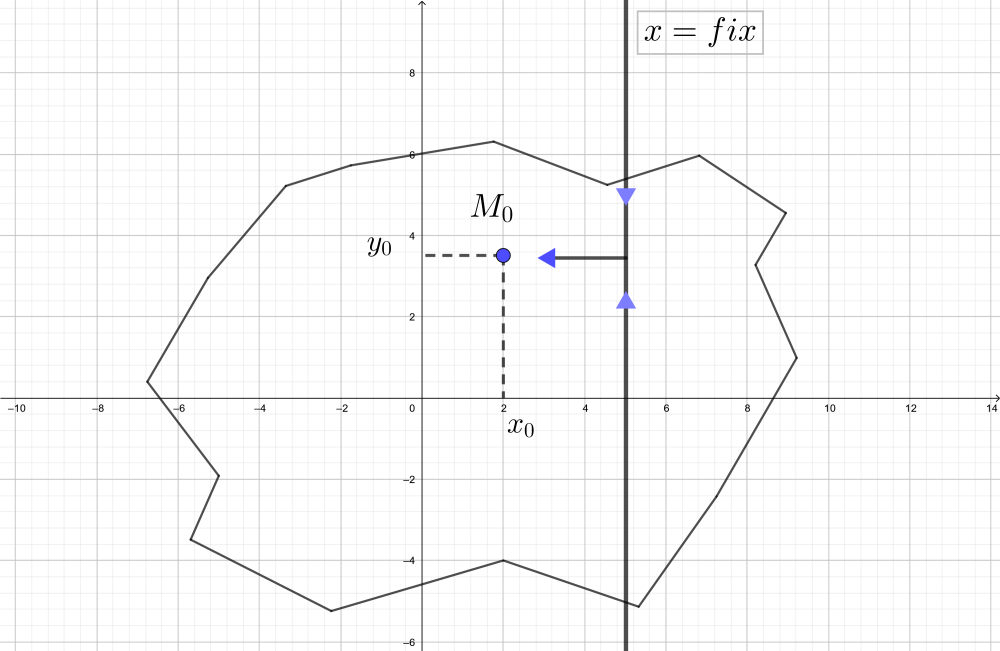
\includegraphics[scale=0.33]{rep-lim-case-a.png}
б) 
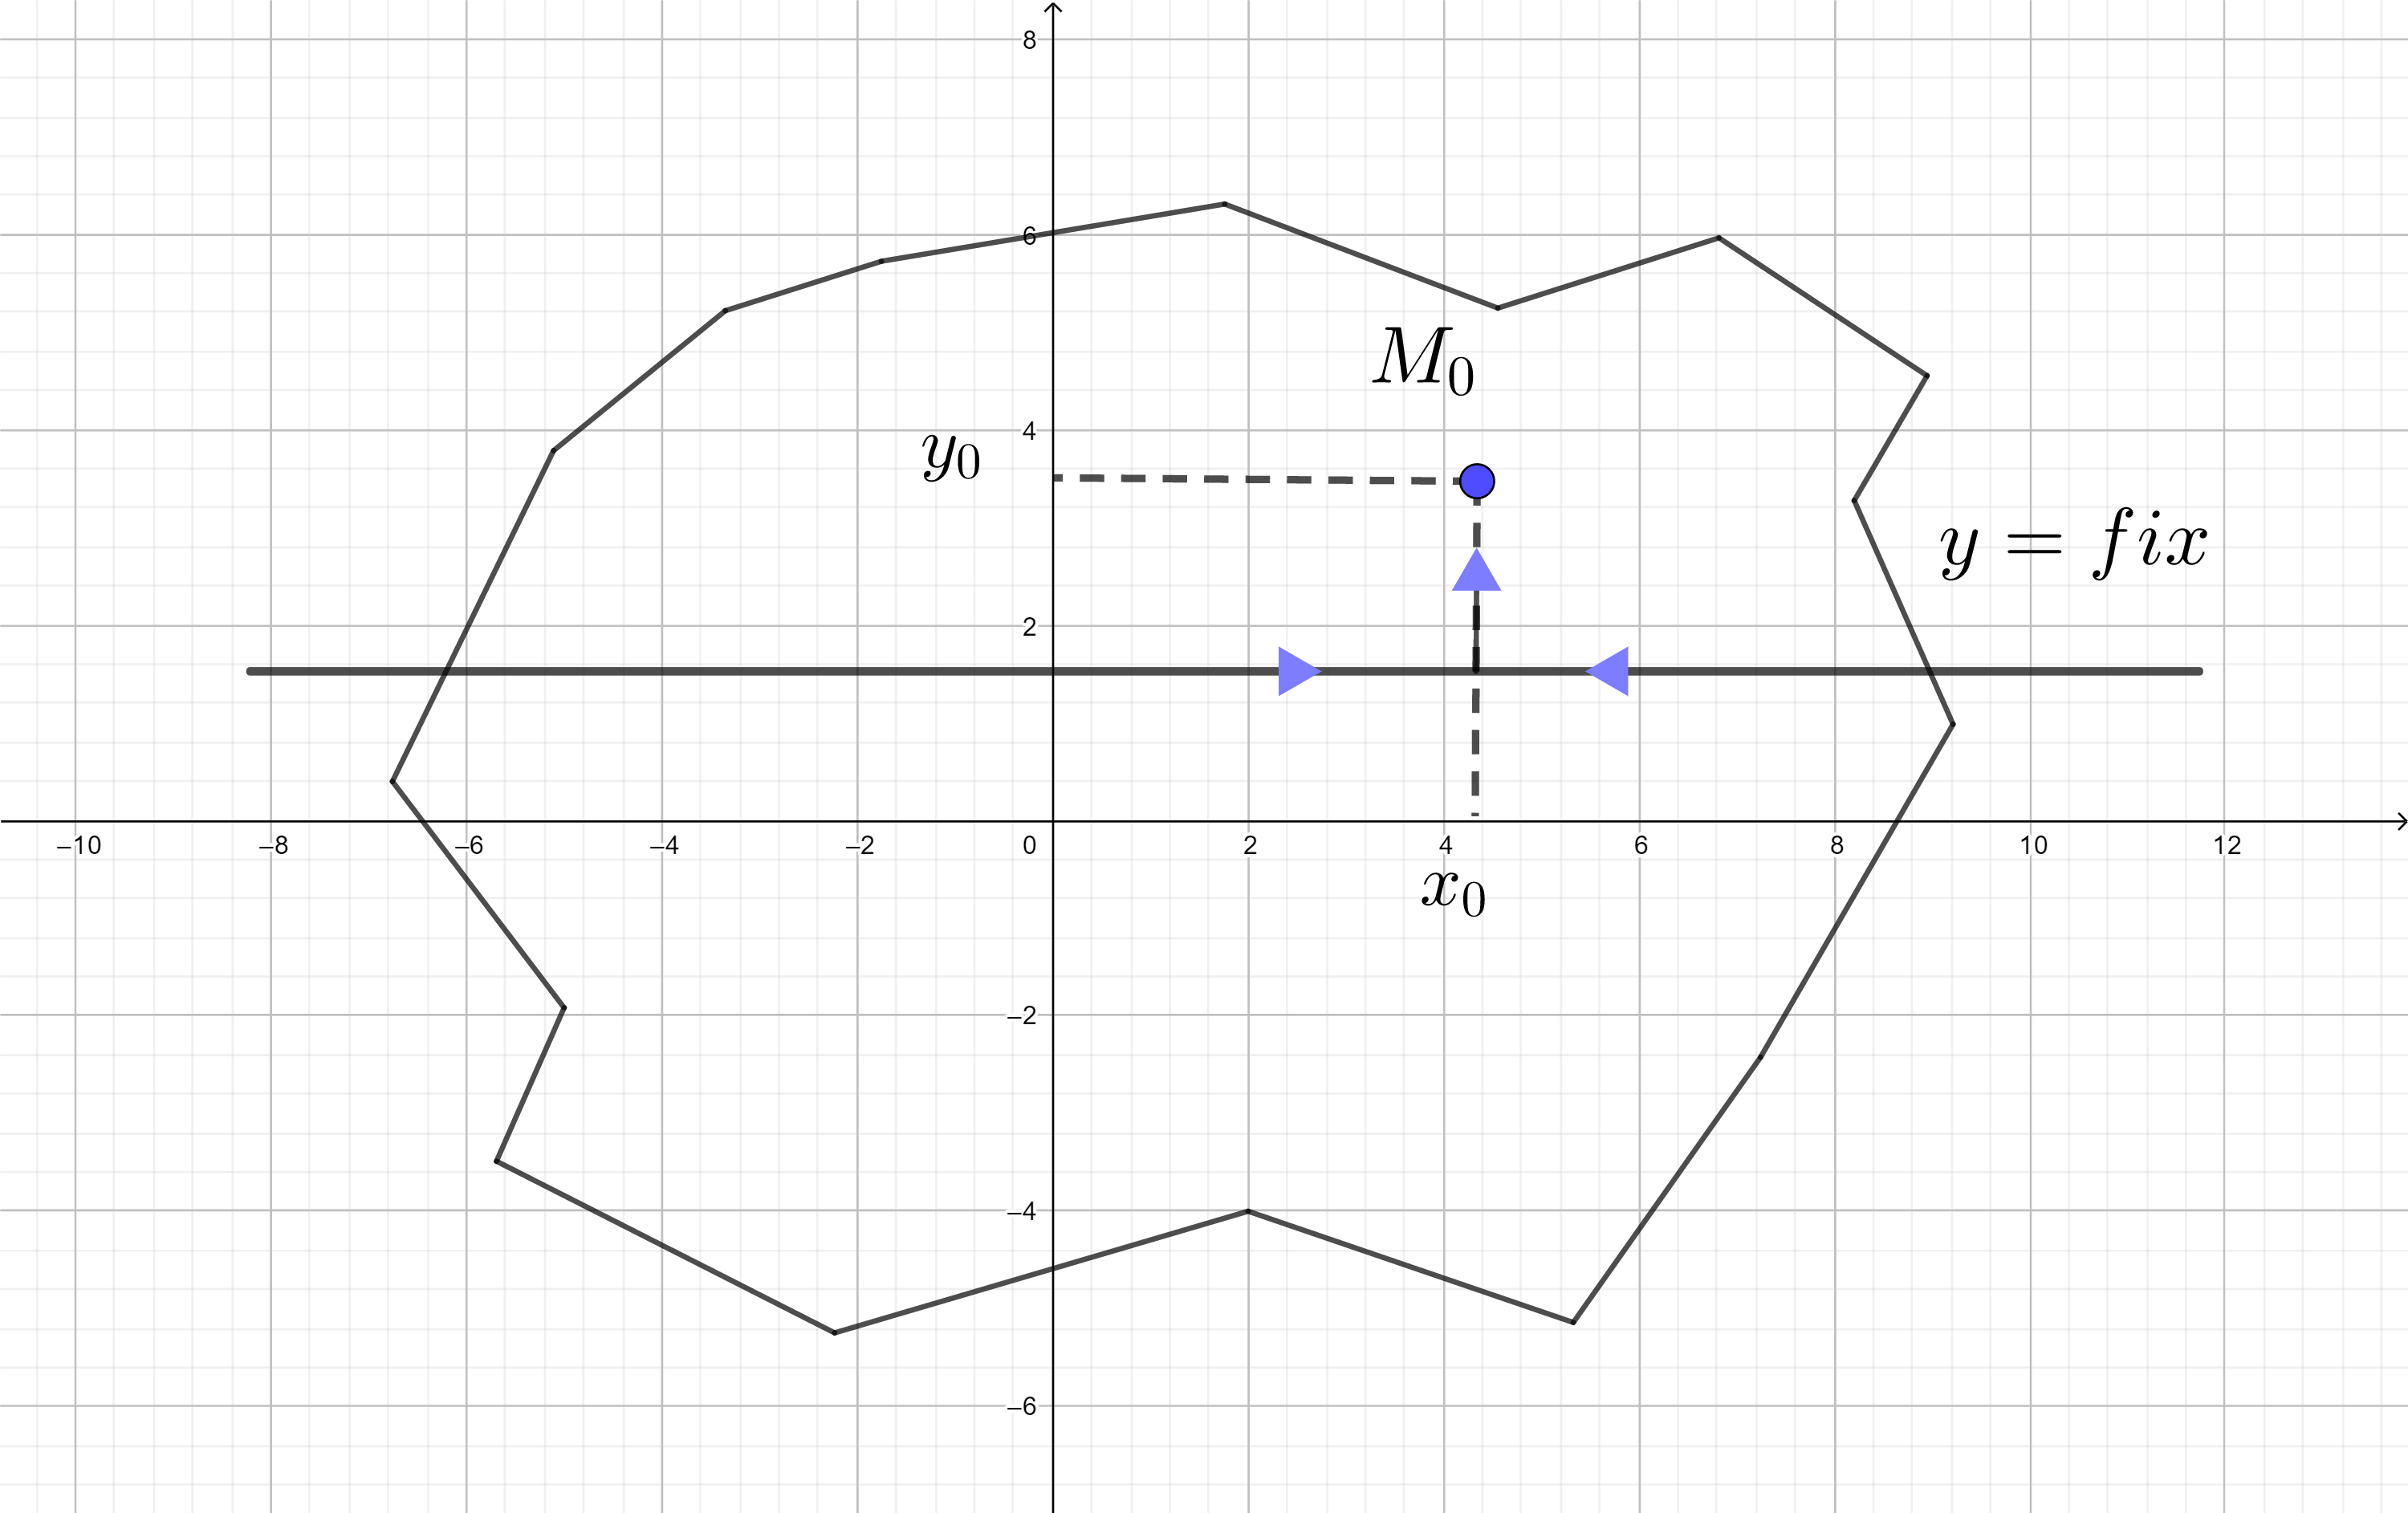
\includegraphics[scale=0.33]{rep-lim-case-b.png}

Кроме \eqref{double-lim} и \eqref{rep-lim} рассматривают частные
пределы пределы Ф2П, когда независимые переменные стемятся к $x_0, y_0$
не произвольным образом, а специальным. Например, по некоторой плоской
кривой $l \subset{D(f)} \subset \R^2$. Можно показать, что если для Ф2П
$\exists$ двойной предел \eqref{double-lim} и $\exists$ повторные
пределы \eqref{rep-lim}, то все они равны между собой. Аналогично и
для частных пределов.

\end{document}
